\documentclass[paper=a4, fontsize=11pt,twoside]{scrartcl} 

\usepackage[a4paper,pdftex]{geometry}	% A4paper margins
\setlength{\oddsidemargin}{5mm}			% Remove 'twosided' indentation
\setlength{\evensidemargin}{5mm}

\usepackage[english]{babel}
\usepackage[protrusion=true,expansion=true]{microtype}	
\usepackage{amsmath,amsfonts,amsthm,amssymb}
\usepackage{graphicx}
\usepackage{listings}
\lstset{
	breaklines=true,
	frame=single,
	captionpos=b
}
\graphicspath{ {images/} }
\usepackage{url}
\usepackage{framed}
\usepackage{subcaption}

% --------------------------------------------------------------------
% Definitions (do not change this)
% --------------------------------------------------------------------
\newcommand{\HRule}[1]{\rule{\linewidth}{#1}} 	% Horizontal rule

\makeatletter							% Title
\def\printtitle{%						
	{\centering \@title\par}}
\makeatother									

\makeatletter							% Author
\def\printauthor{%					
	{\centering \large \@author}}				
\makeatother					

% --------------------------------------------------------------------
% Metadata (Change this)
% --------------------------------------------------------------------
\title{	\normalsize \textsc{Lab 3: State Machines} 	% Subtitle
	\\[2.0cm]								% 2cm spacing
	\HRule{0.5pt} \\						% Upper rule
	\LARGE \textbf{\uppercase{The flow of states in Sequence Detection}}	% Title
	\HRule{2pt} \\ [0.5cm]		% Lower rule + 0.5cm spacing
	\normalsize \today			% Todays date
}

\author{
	Richard Carter\\	
	Clemson University\\	
	Department of Electrical and Computer Engineering\\
	\texttt{rcarte4@clemson.edu} \\
}


\begin{document}
% ------------------------------------------------------------------------------
% Maketitle
% ------------------------------------------------------------------------------
\thispagestyle{empty}		% Remove page numbering on this page

\printtitle					% Print the title data as defined above
\vfill
\printauthor				% Print the author data as defined above
\newpage

% ------------------------------------------------------------------------------
% Abstract
% ------------------------------------------------------------------------------
\thispagestyle{empty}
\vspace*{\fill}
\begin{center}
\begin{Huge}
\section{Abstract} % (fold)
\label{sec:abstract}
\end{Huge}
\end{center}
State machines are incorporated into many of the digital electronics around us. For this project, we attempted to implement a Moore state machine in order to create a digital "lock" system. The design of our state machine followed a traditional design, with the exception of output logic due to our output merely being the encoded representation of our machine's current state. Our testbenches showed that the functionality of our state machine was working as intended, and the DE1 ported hardware worked as planned.

\vspace*{\fill}
% paragraph abstract (end)
\newpage

% ------------------------------------------------------------------------------
% Begin document
% ------------------------------------------------------------------------------

\setcounter{page}{1}		% Set page numbering to begin on this page
\section{Introduction} % (fold)
\label{sec:introduction}
The objective of this project was to construct a Moore state machine that acts as a sequence detector for a set of four different 5-bit sequences. One of these sequences would put the machine into an "UNLOCKED" state, while the other three would put it into a "FALSE UNLOCKED" state. All other sequences would keep the device in a "LOCKED" state. The output of the state machine would simply be the encoded binary representation of the current state of the state machine, and the input to this machine would be the sequence bit, which would be read in on each clock cycle. 

Additionally, an objective of this project was to port the functionality of our Moore state machine to the DE1 Altera board. The clock used for advancing the state machine would be emulated by a push-button input. The input would be determined by a single switch on the board, and the machine's output would be shown using 4 of the board's red LEDs.
% section introduction (end)

\section{DESIGN} % (fold)
\label{sec:design}
	\subsection{OVERALL DESIGN} % (fold)
	\label{sub:overall_design}
	\begin{figure}[h]
		\centering
		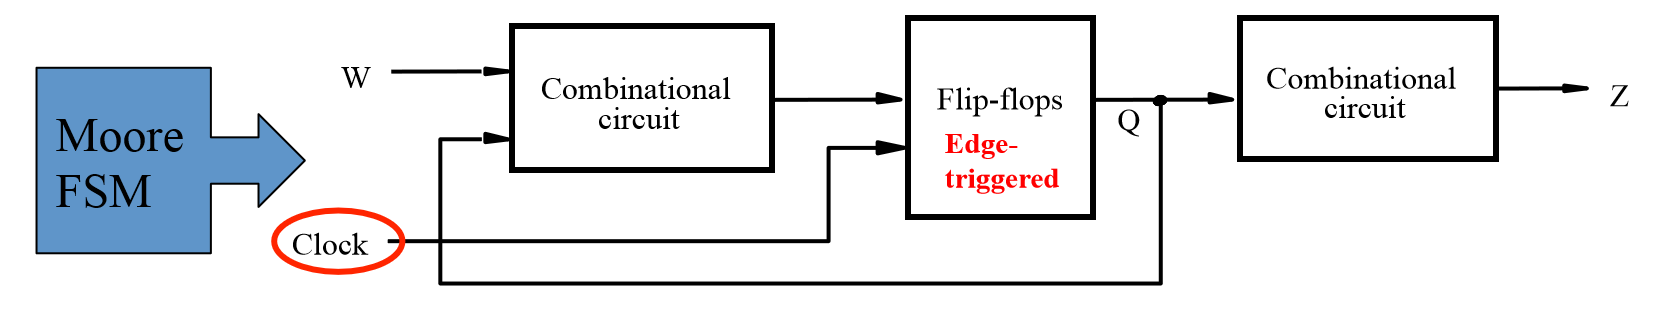
\includegraphics[scale=0.7]{MooreSM.PNG}
		\caption{Moore State Machine Diagram}
		\label{fig:MSM}
	\end{figure}

	Our design started out based on the model of a Moore state machine presented in lecture, which is shown in Figure~\ref{fig:MSM}. However, we soon figured out that the combinational circuit used to determine the output from the data stored in the flip-flop was not needed, as the required output would just be the data stored in the flip-flop (which is the current state of the state machine). Therefore, only the first two blocks are used.
	% subsection overall_design (end)

	\subsection{STATE LOGIC} % (fold)
	\label{sub:state_logic}
	\begin{table}[h]
		\caption{Truth Table for Lock/Unlock State Machine}
		\label{tab:truth}
		\centering
	
		\begin{tabular}{l | l l | l}
		\hline
		\hline
		\textbf{CURRENT} & \multicolumn{2}{c|}{\textbf{NEXT}} & \textbf{OUTPUT} \\
		\hline
		0000 (R) & 1(L1) & 0(R) & 0000 \\
		0001 (L1) & 1(R) & 0(L2) & 0001 \\
		0011 (L2) & 1(L3) & 0(R) & 0011 \\
		0010 (L3) & 1(L5) & 0(L4) & 0010 \\
		0110 (L4) & 1(FU) & 0(FU) & 0110 \\
		0111 (L5) & 1(FU) & 0(U) & 0111 \\
		0101 (ERR) & 1(ERR) & 0(ERR) & 0101	\\
		0100 (FU) & 1(R) & 0(R) & 0100 \\
		1100 (U) & 1(R) & 0(R) & 1100 \\
		\hline
		\end{tabular}
	\end{table}
	The combinational logic used to determine the next state of the state machine is based off of the truth table that we determined for the system, shown in Table~\ref{tab:truth}. State \texttt{R} and states \texttt{L1} through \texttt{L5} are all "LOCKED" states, with the \texttt{ERR} state used for error catching during testing. All locked states will revert back to the \texttt{R} (reset) state if a sequence that cannot lead to a "FALSE UNLOCK" or "UNLOCK" state is detected. The three pre-defined false unlock sequences will all lead to the \texttt{FU} state, and the single unlock sequence will lead to the \texttt{U} state. Both the \texttt{U} and \texttt{FU} states will change to the \texttt{R} state after one clock cycle.

	In VHDL, we accomplished this in an architecture through a when/else assignment~\cite{signal}. Each conditional is representitive of a potential next state given both the incoming input and the current state. A portion of the code for this is shown in Listing~\ref{lst:whenelse}.

	\begin{oframed}
	\begin{lstlisting}[caption={Next State Code},label={lst:whenelse},language=VHDL]
next_state <= L1 when (seq_bit = '1' and prev_state = R) else
	R when (seq_bit = '0' and prev_state = R) else
	R when (seq_bit = '1' and prev_state = L1) else
	L2 when (seq_bit = '0' and prev_state =L1) else
	L3 when (seq_bit = '1' and prev_state = L2) else
	...
	\end{lstlisting}
	\end{oframed}
	% subsection state_logic (end)

	\subsection{STORAGE} % (fold)
	\label{sub:storage}
	For storing the current state, we created the following process shown in Listing~\ref{lst:reg} that will act as our flip-flop. We created a signal with a default value in order to give the state machine a starting state (which is \texttt{R}).
	\begin{oframed}
	\begin{lstlisting}[caption={"Flip Flop" Code},label={lst:reg},language=VHDL]
architecture behav of state_reg is
	signal current_state : std_logic_vector(3 downto 0) := "0000" ;
begin
	state_out <= current_state;

	data_sync : process( clock )
	begin
		if( rising_edge(clock) ) then
			current_state <= state_in;
		end if ;
	end process ; -- data_sync
end architecture ; -- arch
	\end{lstlisting}
	\end{oframed}
	% subsection storage (end)
% section design (end)

\section{TESTING} % (fold)
\label{sec:testing}
In order to confirm full functionality of our state machine, a test bench was created that would simulate a runthrough of all inputs and state changes. These tests can be grouped into three sections, which will be explained in detail in the following sections.
	\subsection{LOCKED STATES} % (fold)
	\label{sub:locked_states}
	\begin{figure}[h]
		\centering
		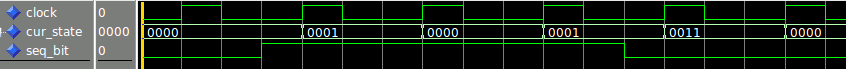
\includegraphics[scale=1.3]{LOCK.png}
		\caption{Timing Diagram of Locked States Testing}
		\label{fig:lock_t}
	\end{figure}
	A pre-defined functionality of our state machine is having incorrect sequences (not FALSE UNLOCKED or UNLOCKED sequences) loop back into the first locked state as soon as it can be determined that the sequence will not lead to \texttt{FU} or \texttt{U} states. Using the truth table shown in Figure~\ref{tab:truth} on page~\pageref{tab:truth}, we determined that the inputs \texttt{0, 11,} and \texttt{100} were the only three input sequences that would cause a state change back to the first locked state (\texttt{R}). Figure~\ref{fig:lock_t} shows our confirmation that our state machine is functioning properly regarding "locked" states.
	% subsection locked_states (end)

	\subsection{FALSE UNLOCKED STATES} % (fold)
	\label{sub:false_unlocked_states}
	We also tested to make sure all \texttt{FU} states could be reached by appropriate sequences. Figure~\ref{fig:FU1} shows our confirmation that the \texttt{10111} sequence results in the \texttt{FU} state and then changes to the \texttt{R} state after a clock cycle. Figures~\ref{fig:FU2} and~\ref{fig:FU3} show the same, but for sequences \texttt{10100} and \texttt{10101} respectively.

	% \begin{figure}[ht]
	% \begin{subfigure}{0.9\textwidth}
	% 	\centering
	% 	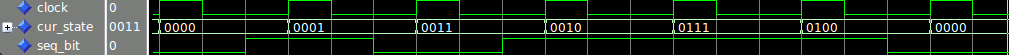
\includegraphics[scale=1.2]{1stFU.png}
	% 	\caption{FU State Testing for \texttt{10111}}
	% 	\label{fig:FU1}
	% \end{subfigure}
	% \begin{subfigure}{0.9\textwidth}
	% 	\centering
	% 	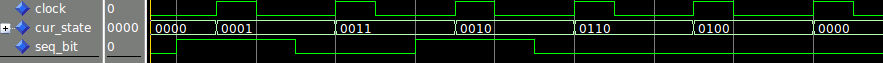
\includegraphics[scale=1.2]{2ndFU.png}
	% 	\caption{FU State Testing for \texttt{10100}}
	% 	\label{fig:FU2}
	% \end{subfigure}
	% \begin{subfigure}{0.9\textwidth}
	% 	\centering
	% 	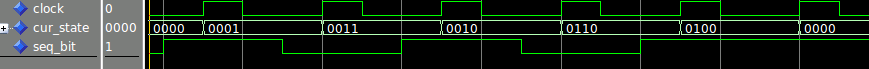
\includegraphics[scale=1.2]{3rdFU.png}
	% 	\caption{FU State Testing for \texttt{10101}}
	% 	\label{fig:FU3}
	% \end{subfigure}
	% \caption{\texttt{FU} State Tests}
	% \end{figure}
	\begin{figure}[ht]
		\centering
		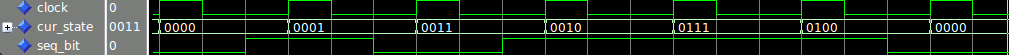
\includegraphics[scale=1.2]{1stFU.png}
		\caption{FU State Testing for \texttt{10111}}
		\label{fig:FU1}
	\end{figure}
	\begin{figure}[ht]
		\centering
		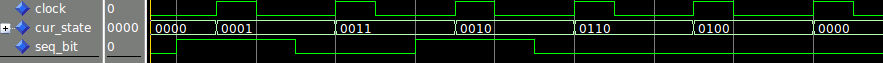
\includegraphics[scale=1.2]{2ndFU.png}
		\caption{FU State Testing for \texttt{10100}}
		\label{fig:FU2}
	\end{figure}
	\begin{figure}[ht]
		\centering
		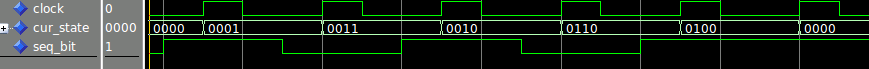
\includegraphics[scale=1.2]{3rdFU.png}
		\caption{FU State Testing for \texttt{10101}}
		\label{fig:FU3}
	\end{figure}


	% subsection false_unlocked_states (end)

	\subsection{UNLOCKED STATE} % (fold)
	\label{sub:unlocked_state}
	\begin{figure}[th]
		\centering
		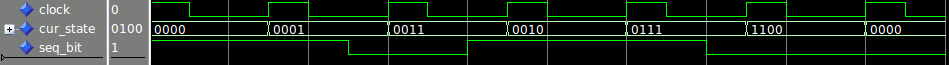
\includegraphics[scale=0.5]{UNLOCK.png}
		\caption{Unlock State Test}
		\label{fig:unlock}
	\end{figure}
	Lastly, the unlock sequence was tested to make sure the \texttt{U} state is achieved properly, as well as being set to \texttt{R} after a clock cycle. Figure~\ref{fig:unlock} shows our confirmation that this functions as planned.
	% subsection unlocked_state (end)
% section testing (end)

\section{Conclusion} % (fold)
\label{sec:conclusion}
The creation of our state machine lock system was a complete success. After creating a wrapper VHDL file for porting purposes, we tested our hardware physically on the DE1 board and it worked as planned. If there were any lessons to be learned from this project, it would be the value of running test benches before porting to physical hardware. Due to not having an initial state stored in our flip-flop, there may have been undefined behavior in our state machine had we just ported it from the get-go.
% section conclusion (end)



\bibliographystyle{abbrv}
\bibliography{myreference}

% \section{Appendix}\label{appendix}

\end{document}
This is never printed